%% Beispiel-Präsentation
\documentclass[de,16:9]{sdqbeamer} 
 
%% Titelbild
\titleimage{banner_2020_kit}

%% Gruppenlogo
% \grouplogo{SDQ-Logo-new.png} 
\grouplogo{}

%% Gruppenname
% \groupname{Abteilungs-, KIT-Fakultäts-, Institutsbezeichnung}

% Beginn der Präsentation

\title[Proseminar: Optimierungsansätze für Adaptionsstrategien in SAS]{Proseminar: Optimierungsansätze für Adaptionsstrategien in SAS}
\subtitle[Betreuerin: Dipl.-Inform. Martina Rapp]{Betreuerin: Dipl.-Inform. Martina Rapp}
\author[Tim Engbrocks]{Tim Engbrocks}

\date[22.\,07.\,2021]{22.\,07.\,2021}

% Literatur 
 
\usepackage[citestyle=authoryear,bibstyle=numeric,hyperref,backend=biber,maxcitenames=2]{biblatex}
\addbibresource{presentation.bib}
\bibhang1em

\begin{document}

%Titelseite
\KITtitleframe

%Inhaltsverzeichnis
\begin{frame}{Inhaltsverzeichnis}
\tableofcontents
\end{frame}

\section{Einführung}

\begin{frame}{Die Komplexität von Software}
	\begin{center}
		Die Komplexität von Software steigt stetig. \\
		\glqq The looming software crisis \grqq - IBM, 2001
	\end{center}
	\medskip
	\begin{itemize}
		\item Moderne Sprachmodelle: 
		\begin{itemize}
			\item GPT-3 von OpenAI: 175 Milliarden Parameter [\cite{GPT3}]
			\item Turing-NLG von Microsoft: 17 Milliarden Parameter [\cite{TuringNLG}]
		\end{itemize}
		\item Teslas Autopilot AI sagt 10.000 Parameter vorraus [\cite{TeslaAutopilot}]
	\end{itemize}
\end{frame}

\begin{frame}{Netflix Microservice Architektur}
	\begin{center}
		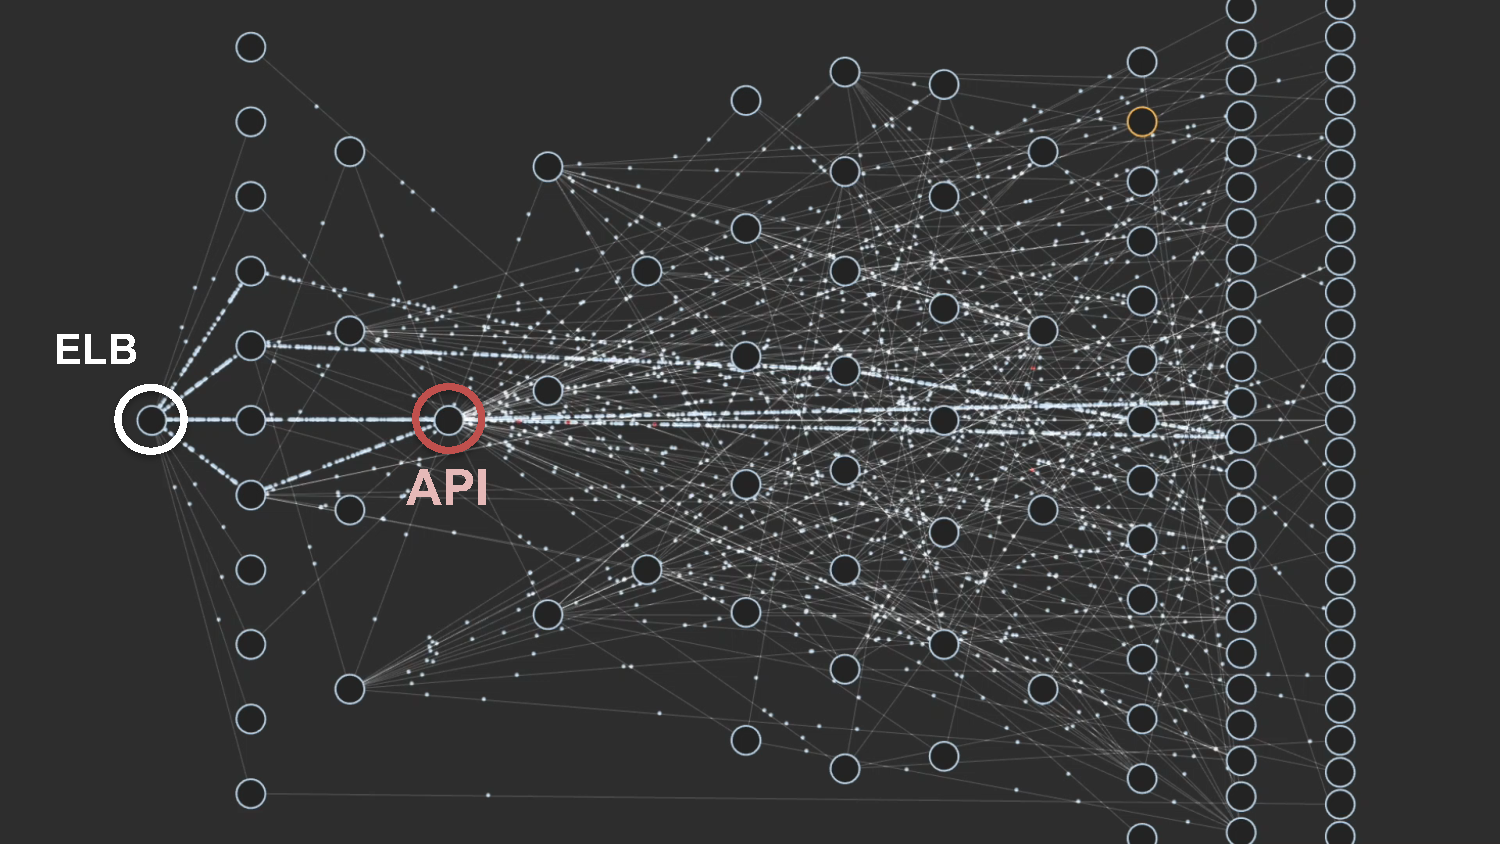
\includegraphics[width=0.65\textwidth]{sources/Mastering Chaos.pdf}
		[\cite{JoshQCon}]
	\end{center}
\end{frame}

\begin{frame}{Die Lösung: Autonomes Management}
	\begin{center}
		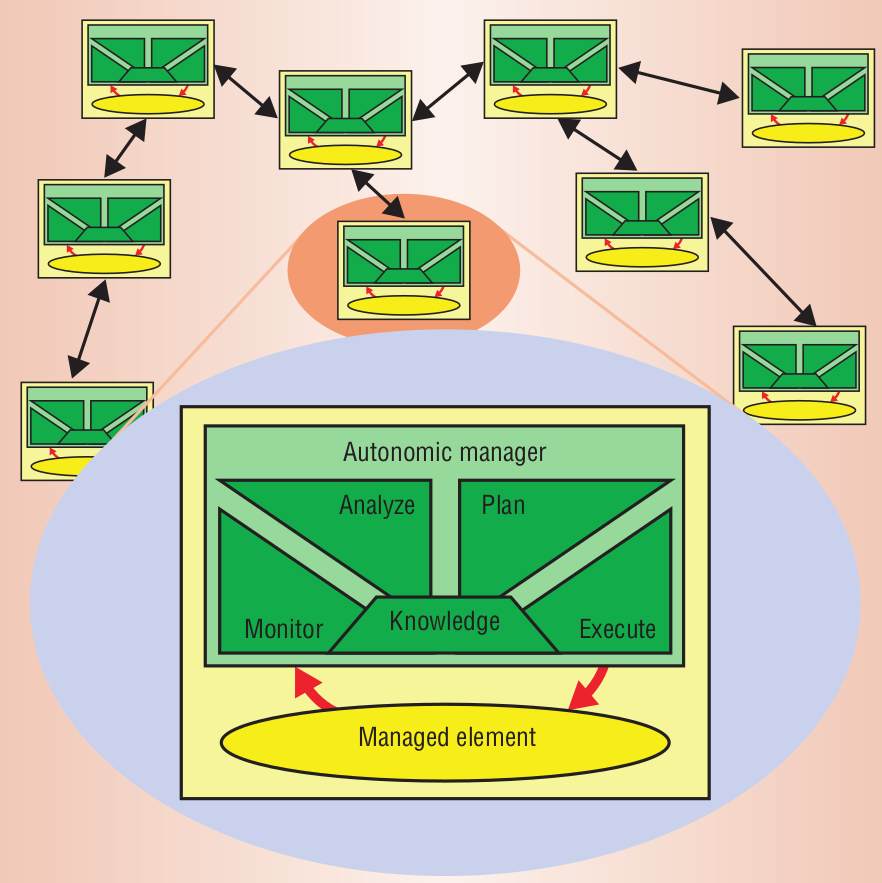
\includegraphics[height=0.7\textheight]{sources/MAPEK.png}
		[\cite{VisionOfAutonomicComputing}]
	\end{center}
\end{frame}

\section{Selbstadaptive Systeme}

\begin{frame}{Definition}
	\begin{greenblock}{Selbstadaptives System}
		Ein System, das sich autonom steuert durch das:
		\begin{itemize}
			\item \textit{Beobachten} des Kontextes
			\item \textit{Analysieren} von Veränderungen
			\item \textit{Planen} von Anpassungen
			\item \textit{Ausführen} von Anpassungen
		\end{itemize}
	\end{greenblock}
\end{frame}

\begin{frame}{Beispiel: kommerzielles Web Angebot}
	\begin{itemize}
		\item Szenario: System Administrator eines kommerziellen Web Angebots.
		\item Tägliche Aufgabe: System Parameter X basierend auf Metrik Y anpassen.
	\end{itemize}
	\medskip
	Dieses Szenario kann von einem Selbstadaptiven System profitieren:
	\begin{itemize}
		\item Generelle Anpassungs Regel:
		Wenn die Metrik Y den Schwellwert Z übersteigt: Passe den System Parameter X an
		\item Beispiel: Wenn die Serverlast zu hoch wird: Starte einen zusätzlichen Server
	\end{itemize}
\end{frame}

\begin{frame}{Selbstadaptive Systeme klassifizieren}
	\begin{center}
		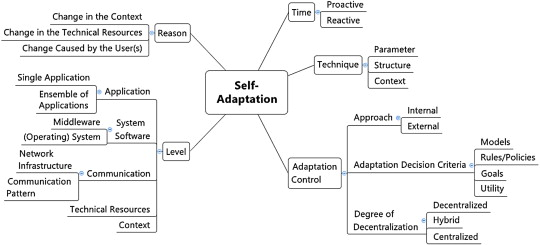
\includegraphics[width=0.8\textwidth]{sources/KrupitzerTaxonomy.jpg}
		[\cite{SurveyOnEngineeringApproaches}]
	\end{center}
\end{frame}

\begin{frame}{Grenzen von Selbstadaptiven Systemen}
	\begin{center}
		\Large \textbf{Unsicherheit}
		\\ \medskip
		Änderungen im Kontext $\Rightarrow$ Unerwartete Ergebnisse von Anpassungen
	\end{center}
\end{frame}

\section{Optimierungsansätze}

\begin{frame}{Optimierungen für Selbstadaptive Systeme}
	Der meist verwendete Optimierungsansatz:
	\begin{itemize}
		\item Dynamisch Adaptations Regeln anpassen
	\end{itemize}
	\medskip
	Viele Ansätze verwenden maschinelles lernen, um neue Regeln zu generieren
	oder bestehende anzupassen. \\
	\medskip
	Andere Aspekte des Systems können auch optimiert werden:
	\begin{itemize}
		\item Adaptations Steuerung: Wie
		\item Ebene: Wo
		\item Methode: Was
	\end{itemize}
\end{frame}

\section{Klassifizierung}

\begin{frame}{Eine Klassifizierung entwicklen}
	Die Klassifizierung basiert auf drei Konzepten:
	\begin{itemize}
		\item Reflektive Systeme [\cite{FORMS}]
		\item Die 6W Fragen [\cite{LandscapeAndResearchChallenges}]
		\begin{itemize}
			\item Wieso, Wo, Wann, Was, Wer und Wie
		\end{itemize}
		\item Die Klassifizierung von Selbstadaptiven Systemen [\cite{SurveyOnEngineeringApproaches}]
	\end{itemize}
\end{frame}

\begin{frame}{Vorschlag einer Klassifizierung}
	\begin{center}
		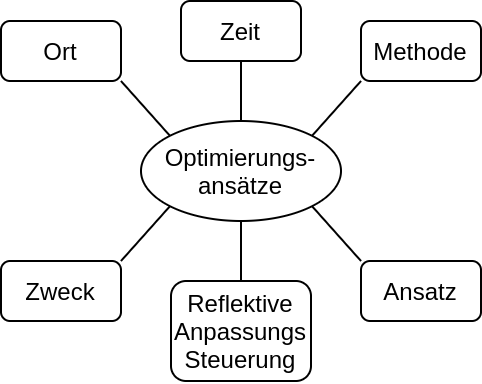
\includegraphics[width=.45\textwidth]{sources/ClassificationProposal-Proposal_DE.png}
	\end{center}
\end{frame}

\begin{frame}{Klassifizierung - Ort}
	\begin{columns}
		\column{.5\textwidth} \begin{center}
			\begin{greenblock}{Ort}
				\begin{itemize}
					\item Adaptations Steuerung
					\item Ebene
					\item Methode
				\end{itemize}
			\end{greenblock}
		\end{center}
		\column{.5\textwidth} \begin{center}
			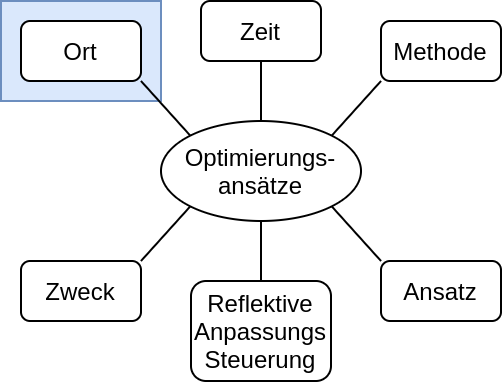
\includegraphics[width=0.6\textwidth]{sources/ClassificationProposal-Proposal_DE_Location.png}
		\end{center}
	\end{columns}
\end{frame}

\begin{frame}{Klassifizierung - Zeit}
	\begin{columns}
		\column{.5\textwidth} \begin{center}
			\begin{greenblock}{Zeit}
				\begin{itemize}
					\item Entwurfsphase
					\item Laufzeit / Online Phase
					\item Offline Phase
				\end{itemize}
			\end{greenblock}
		\end{center}
		\column{.5\textwidth} \begin{center}
			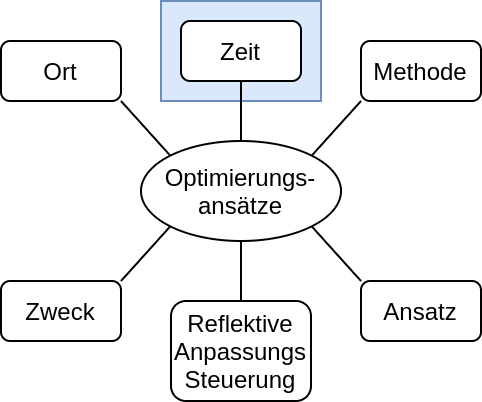
\includegraphics[width=0.6\textwidth]{sources/ClassificationProposal-Proposal_DE_Time.png}
		\end{center}
	\end{columns}
\end{frame}

\begin{frame}{Klassifizierung - Methode}
	\begin{columns}
		\column{.5\textwidth} \begin{center}
			\begin{greenblock}{Methode}
				\begin{itemize}
					\item Adaptations Regeln
					\item Wissen
					\item Adaptations Methode
					\item Ebene
				\end{itemize}
			\end{greenblock}
		\end{center}
		\column{.5\textwidth} \begin{center}
			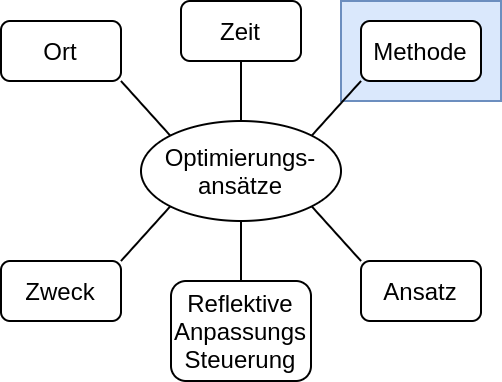
\includegraphics[width=0.6\textwidth]{sources/ClassificationProposal-Proposal_DE_Technique.png}
		\end{center}
	\end{columns}
\end{frame}

\begin{frame}{Klassifizierung - Zweck}
	\begin{columns}
		\column{.5\textwidth} \begin{center}
			\begin{greenblock}{Zweck}
				\begin{itemize}
					\item Vorhandenes Wissen anpassen
					\item Adaptations Regeln an die neue Umgebung anpassen
					\item Ein Ziel erfüllen
					\item Eine Nutzenfunktion maximieren/minimieren
				\end{itemize}
			\end{greenblock}
		\end{center}
		\column{.5\textwidth} \begin{center}
			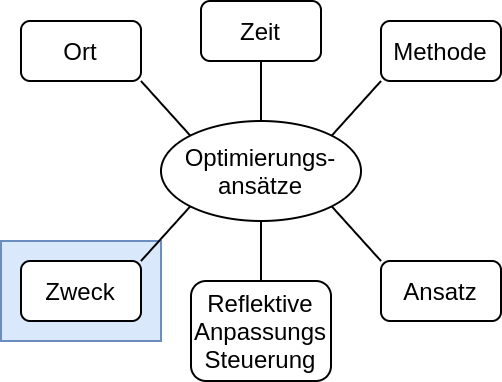
\includegraphics[width=0.6\textwidth]{sources/ClassificationProposal-Proposal_DE_Purpose.png}
		\end{center}
	\end{columns}
\end{frame}

\begin{frame}{Klassifizierung - Ansatz}
	\begin{columns}
		\column{.5\textwidth} \begin{center}
			\begin{greenblock}{Ansatz}
				\begin{itemize}
					\item Intern / Extern
					\item Grad der Dezentralisierung:
					\begin{itemize}
						\item Komplett zentral
						\item Komplett dezentral
						\item Sowohl zentral als auch dezentral
					\end{itemize}
				\end{itemize}
			\end{greenblock}
		\end{center}
		\column{.5\textwidth} \begin{center}
			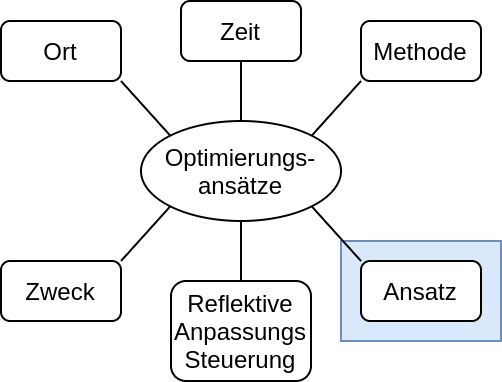
\includegraphics[width=0.6\textwidth]{sources/ClassificationProposal-Proposal_DE_Approach.png}
		\end{center}
	\end{columns}
\end{frame}

\begin{frame}{Klassifizierung - Reflektive Anpassungs Steuerung}
	\begin{columns}
		\column{.5\textwidth} \begin{center}
			\begin{greenblock}{Reflektive Anpassungs Steuerung}
				\begin{itemize}
					\item Modelle anpassen
					\item Adaptations Regeln anpassen
					\item Ziele erfüllen
					\item Nutzenfunktionen maximieren/minimieren
				\end{itemize}
			\end{greenblock}
		\end{center}
		\column{.5\textwidth} \begin{center}
			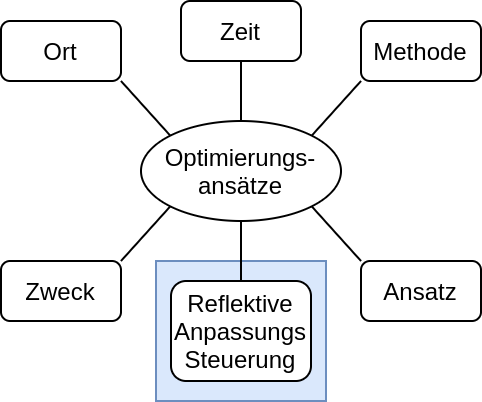
\includegraphics[width=0.6\textwidth]{sources/ClassificationProposal-Proposal_DE_RAC.png}
		\end{center}
	\end{columns}
\end{frame}

\begin{frame}{Vorschlag einer Klassifizierung}
	\begin{center}
		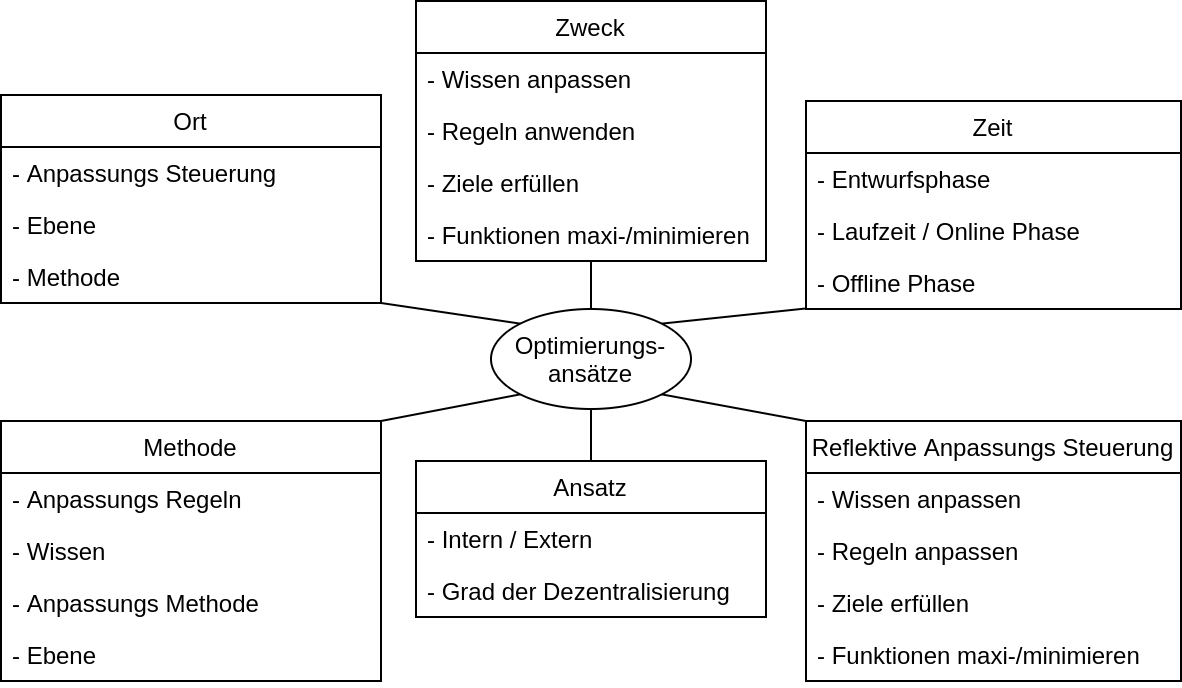
\includegraphics[width=.6\textwidth]{sources/ClassificationProposal-WithDimensions_DE.png}
	\end{center}
\end{frame}

\section{Fazit}

\begin{frame}{Schlussfolgerungen}
	Nur wenige Optimierungsansätze verwenden:
	\begin{itemize}
		\item Zeit: Entwurfsphase und Offline Phase
		\item Ort: Ebene und Methode
		\item Ansatz: Dezentral
	\end{itemize}
\end{frame}

\begin{frame}{Weitere Forschung}
	Folgende Bereiche benötigen weitere Forschung:
	\begin{itemize}
		\item Die vorherigen Dimensionen erforschen
		\item Eine Methode, um den Nutzen von Optimierungsansätzen zu quantifizieren
		\item Selbstadaptive Systeme und Optimierungsansätze, die unabhängig von der Domäne sind
	\end{itemize}
\end{frame}

\appendix
\beginbackup

\begin{frame}[allowframebreaks]{Literatur}
\printbibliography
\end{frame}

\backupend

\end{document}